% Editable standalone vector figure extracted from spectra.tex.
% Source slide 4; figure 03; native embedded fonts.
% Compile with LuaLaTeX from this directory, or run ../export_figures.py.
\documentclass[tikz,border=0pt]{standalone}
% Shared editable preamble for standalone, Nature-style vector figures.
% Text remains embedded and searchable. This is a house-style target, not a
% claim of acceptance or of satisfying every journal's submission checklist.
\usepackage{fontspec}
\setmainfont{LiberationSans}[
  Path=../../shared/assets/,Extension=.ttf,
  UprightFont=*-Regular,BoldFont=*-Bold,ItalicFont=*-Italic,BoldItalicFont=*-BoldItalic]
\setsansfont{LiberationSans}[
  Path=../../shared/assets/,Extension=.ttf,
  UprightFont=*-Regular,BoldFont=*-Bold,ItalicFont=*-Italic,BoldItalicFont=*-BoldItalic]
\setmonofont{LiberationSans}[
  Path=../../shared/assets/,Extension=.ttf,
  UprightFont=*-Regular,BoldFont=*-Bold,ItalicFont=*-Italic,BoldItalicFont=*-BoldItalic]
\usepackage{unicode-math}
\setmathfont{Latin Modern Math}
\DeclareMathSizes{5.9}{6}{5}{5}
\DeclareMathSizes{6}{6}{5}{5}
\usepackage{tikz}
\usetikzlibrary{arrows.meta,calc,positioning,patterns,decorations.pathreplacing,matrix}
\usepackage{graphicx}
\usepackage{xcolor}
\pagecolor{white}
\definecolor{ink}{HTML}{202020}
\definecolor{paper}{HTML}{FFFFFF}
\definecolor{muted}{HTML}{494949}
\definecolor{line}{HTML}{808080}
\definecolor{soft}{HTML}{F0F0F0}
\hyphenpenalty=10000\exhyphenpenalty=10000
\newcommand{\figurefont}{\sffamily\fontsize{5.9}{7.4}\selectfont}
\newcommand{\figuremathfont}{\sffamily\fontsize{6}{7.5}\selectfont}
\newcommand{\brandmedium}{\bfseries}
\renewcommand{\normalsize}{\figurefont}
\renewcommand{\small}{\figurefont}
\renewcommand{\footnotesize}{\figurefont}
\renewcommand{\scriptsize}{\figurefont}
\renewcommand{\tiny}{\figurefont}
\renewcommand{\large}{\figurefont}
\renewcommand{\Large}{\figurefont}
\renewcommand{\LARGE}{\figurefont}
\renewcommand{\huge}{\figurefont}
\renewcommand{\Huge}{\figurefont}
\tikzset{
  every path/.style={line width=.55pt},
  every node/.style={font=\figurefont,text=ink},
  arr/.style={-{Latex[length=1.5mm,width=1mm]},line width=.55pt,draw=ink},
  thinarr/.style={-{Latex[length=1.3mm,width=.9mm]},line width=.55pt,draw=ink},
  box/.style={draw=ink,line width=.55pt,fill=white,minimum height=.85cm,align=center,inner sep=3pt},
  ghost/.style={draw=muted,dashed,fill=soft},
  tag/.style={font=\figurefont,text=muted},
  equ/.style={font=\figuremathfont},
  small/.style={font=\figurefont},
  body/.style={font=\figurefont},
  tinytext/.style={font=\figurefont}
}
\newcommand{\txt}[4]{\node[anchor=north west,align=left,text width=#3cm] at (#1,#2) {#4};}
\newcommand{\smalltxt}[4]{\node[anchor=north west,align=left,text width=#3cm,small] at (#1,#2) {#4};}
\newcommand{\eqn}[4][6]{\node[anchor=north west,font=\figuremathfont] at (#2,#3) {$\displaystyle #4$};}
\newcommand{\diagramblock}[5]{\node[box,minimum width=#3cm,text width=#3cm,minimum height=#4cm] at (#1,#2) {#5};}
% Scale coordinates, not text: all labels retain one final publication size.
\newcommand{\spectrum}[3]{\begin{scope}[shift={(#1,#2)}]
  \draw[muted] (0,0)--({3.6*#3},0);
  \draw[muted] (0,0)--(0,{1.9*#3});
  \foreach \x/\h in {.25/.18,.49/.46,.68/1.42,.87/.37,1.08/.74,1.31/.31,1.57/1.78,1.76/.46,1.96/.19,2.17/1.1,2.37/.57,2.57/.31,2.88/.76,3.21/.23,3.4/.38}{
    \draw[ink] ({\x*#3},0)--({\x*#3},{\h*#3});}
  \foreach \x in {.6,1.2,1.8,2.4,3.0}{\draw[ink] ({\x*#3},0)--+(0,{-.06*#3});}
  \foreach \y in {.45,.9,1.35,1.8}{\draw[ink] (0,{\y*#3})--+({-.06*#3},0);}
  \foreach \x/\lab in {0/0,1.8/45,3.6/90}{\node[anchor=north,font=\figurefont] at ({\x*#3},{-.08*#3}) {\lab};}
  \foreach \y/\lab in {0/0,.9/0.5,1.8/1.0}{\node[anchor=east,font=\figurefont] at ({-.08*#3},{\y*#3}) {\lab};}
  \node[anchor=north east,font=\figurefont] at ({3.6*#3},{-.45*#3}) {$m/z$ (Th)};
  \node[anchor=south west,font=\figurefont] at (0,{1.96*#3}) {Relative intensity (a.u.)};
\end{scope}}
\newcommand{\molecule}[3]{\begin{scope}[shift={(#1,#2)}]
  \draw[ink] (0,{#3})--({.866*#3},{.5*#3})--({.866*#3},{-.5*#3})--(0,{-#3})--({-.866*#3},{-.5*#3})--({-.866*#3},{.5*#3})--cycle;
  \draw[ink] ({.68*#3},{.4*#3})--({.68*#3},{-.4*#3});
  \draw[ink] ({-.7*#3},{-.44*#3})--({-.02*#3},{-.83*#3});
  \draw[ink] ({-.7*#3},{.44*#3})--({-.02*#3},{.83*#3});
  \draw[ink] (0,{#3})--(0,{1.55*#3});
  \node[font=\figurefont] at (0,{1.77*#3}) {OH};
\end{scope}}
\newcommand{\peaktokens}[3]{\foreach \i in {0,...,5}{\pgfmathsetmacro{\xx}{#1+\i*.36}\draw[fill=#3,draw=ink] (\xx,#2) rectangle +(.24,.6);}}
\newcommand{\E}{\mathbb E}
\newcommand{\R}{\mathbb R}
\newcommand{\sg}{\operatorname{stopgrad}}
\newcommand{\LN}{\operatorname{LN}}
\newcommand{\softmax}{\operatorname{softmax}}

\begin{document}
\figurefont
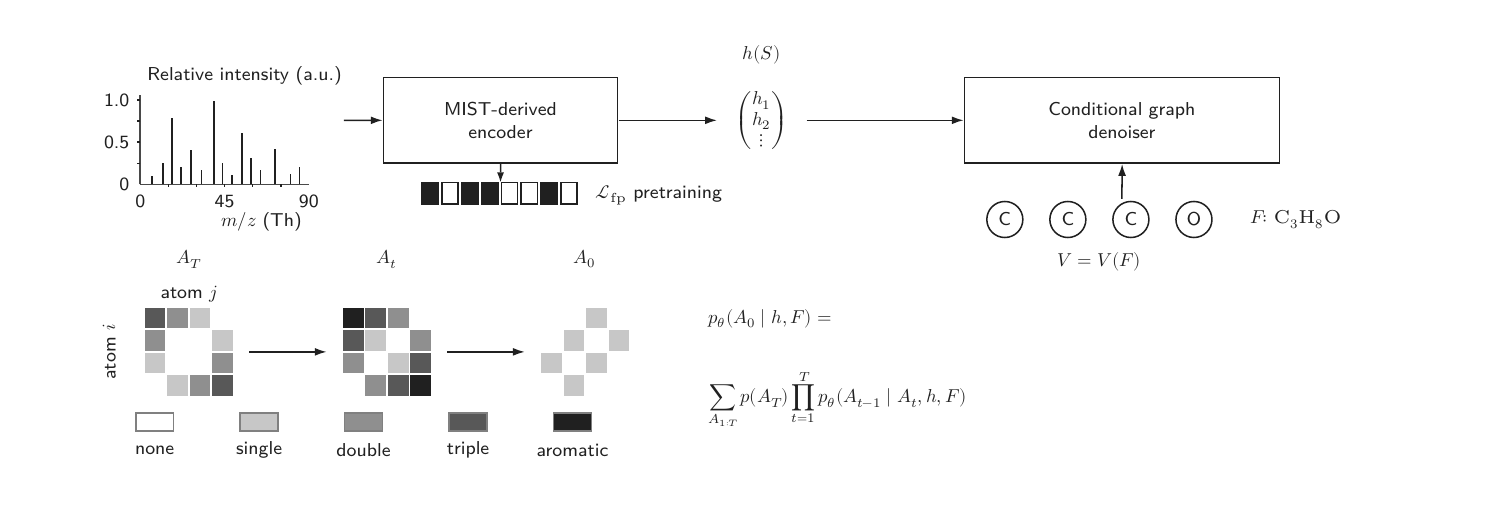
\begin{tikzpicture}[x=1cm,y=1cm,scale=1.14375,transform shape]
% Spectrum -> encoder -> continuous representation -> graph denoiser.
\spectrum{1.25}{5.11}{.52}
\node[box,minimum width=2.6cm,text width=2.3cm,minimum height=.95cm,inner sep=4pt] (diffencoder) at (5.25,5.82) {MIST-derived\\encoder};
\node[inner sep=0,font=\figurefont] (diffembedding) at (8.15,5.82) {$\begin{pmatrix}h_1\\[-1pt]h_2\\[-1pt]\vdots\end{pmatrix}$};
\node[small,inner sep=0] at (8.15,6.55) {$h(S)$};
\node[box,minimum width=3.5cm,text width=3.2cm,minimum height=.95cm,inner sep=4pt] (diffdecoder) at (12.15,5.82) {Conditional graph\\denoiser};
\draw[arr] (3.51,5.82)--(diffencoder.west);
\draw[arr] (diffencoder.east)--([xshift=-.20cm]diffembedding.west);
\draw[arr] ([xshift=.20cm]diffembedding.east)--(diffdecoder.west);
% Fingerprint supervision is an auxiliary pretraining branch, not the inference condition.
\foreach \i/\shade in {0/100,1/0,2/100,3/100,4/0,5/0,6/100,7/0}{\draw[draw=ink,line width=.55pt,fill=ink!\shade] (4.38+\i*.22,4.89) rectangle +(.18,.24);}
\draw[thinarr,dashed] (diffencoder.south)--(5.25,5.13);
\node[small,anchor=west,inner sep=0] at (6.30,4.99) {$\mathcal L_{\rm fp}$ pretraining};
% An illustrative fixed heavy-atom inventory, with no learned atom identities.
\foreach \x/\label/\name in {10.85/C/fixedA,11.55/C/fixedB,12.25/C/fixedC,12.95/O/fixedD}{\node[circle,draw=ink,line width=.55pt,minimum size=.4cm,inner sep=0,small] (\name) at (\x,4.72) {\label};}
\draw[arr] (12.15,4.95)--(diffdecoder.south);
\node[small,inner sep=0] at (14.08,4.72) {$F{:}\ \mathrm C_3\mathrm H_8\mathrm O$};
\node[small,inner sep=0] at (11.90,4.25) {$V=V(F)$};
% The matrix trajectory uses that fixed atom order.
\foreach \i/\x in {0/1.30,1/3.50,2/5.70}{
 \node[small] at (\x+.49,4.28) {$A_{\ifnum\i=0 T\else\ifnum\i=1 t\else0\fi\fi}$};
 \foreach \a in {0,...,3}{\foreach \b in {0,...,3}{\pgfmathtruncatemacro{\shade}{ifthenelse(\a==\b,0,ifthenelse(\i==2,ifthenelse(abs(\a-\b)==1,25,0),mod(\a+\b+\a*\b+\i,5)*25))}\fill[ink!\shade] (\x+\a*.25,2.76+\b*.25) rectangle +(.23,.23);}}
}
\draw[arr] (2.46,3.25)--(3.32,3.25);\draw[arr] (4.66,3.25)--(5.52,3.25);
\node[small,rotate=90] at (.91,3.25) {atom $i$};\node[tinytext] at (1.79,3.89) {atom $j$};
\foreach \x/\shade/\lab in {1.2/0/none,2.36/25/single,3.52/50/double,4.68/75/triple,5.84/100/aromatic}{\draw[fill=ink!\shade,draw=line,line width=.55pt] (\x,2.37) rectangle +(.42,.2);\node[tinytext,font=\figurefont] at (\x+.21,2.16) {\lab};}
\node[anchor=west,inner sep=0,font=\figurefont] at (7.55,3.62) {$\displaystyle p_\theta(A_0\mid h,F)=$};
\node[anchor=west,inner sep=0,font=\figurefont] at (7.55,2.72) {$\displaystyle\sum_{A_{1:T}}p(A_T)\prod_{t=1}^{T}p_\theta(A_{t-1}\mid A_t,h,F)$};
% Fixed canvas: 183 x 60.046875 mm. No clipping: overflow is audited.
\pgfresetboundingbox
\path[use as bounding box] (0,1.6) rectangle (16,6.85);
\end{tikzpicture}
\end{document}
